% !TEX spellcheck = en_US

% !TEX root = elastophi-report.tex


\section{Results}

%\begin{figure}[p]
%\centering
%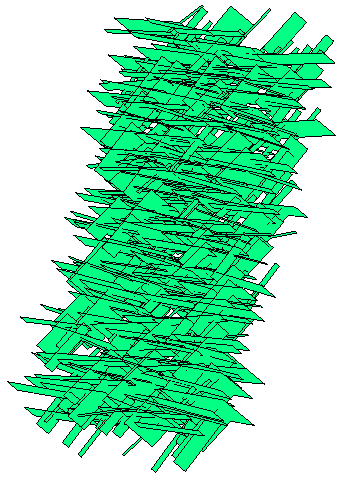
\includegraphics[width=0.4\textwidth]{../images/visu_maillage450Fracs.png}
%\caption{maillage450Fracs}
%\label{fig:maillage450Fracs}
%\end{figure}


\begin{figure}[p]
\centering
\subfloat[][Mesh.]
   {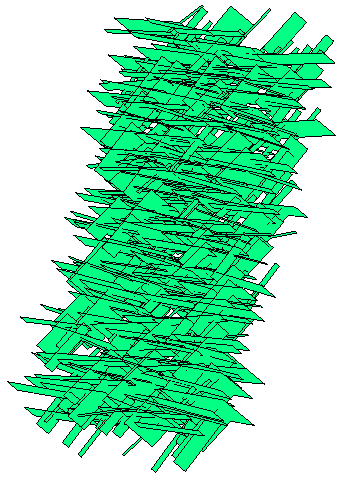
\includegraphics[width=.3\textwidth]{../images/visu_maillage450Fracs.png}} \quad
\subfloat[][Matrix compression for $\eta=1, \varepsilon=0.9$.]
   {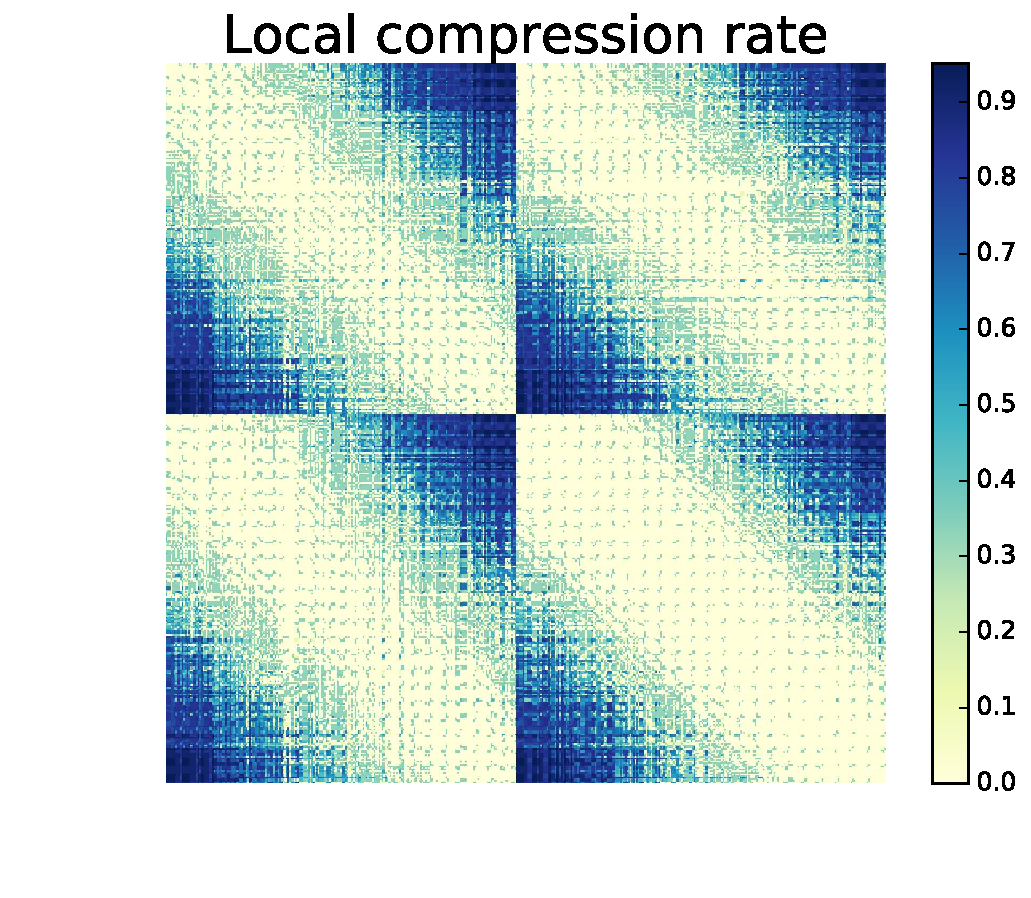
\includegraphics[width=.4\textwidth]{../images/graphe_mapp_output_local_comp_1_0,9_matrice450Fracs.pdf}} \\
\subfloat[][Matrix compression for $\eta=10, \varepsilon=0.9$.]
   {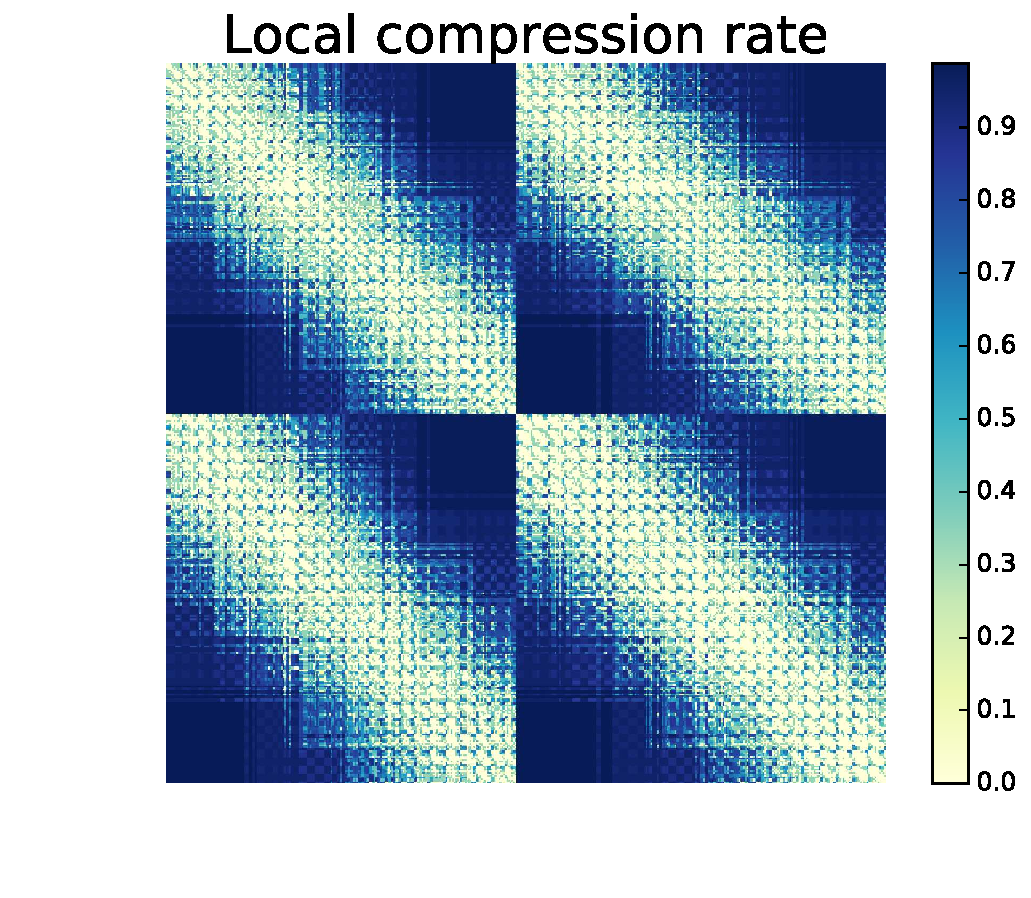
\includegraphics[width=.4\textwidth]{../images/graphe_mapp_output_local_comp_10_0,9_matrice450Fracs.pdf}}
\subfloat[][Matrix compression for $\eta=10, \varepsilon=1$.]
   {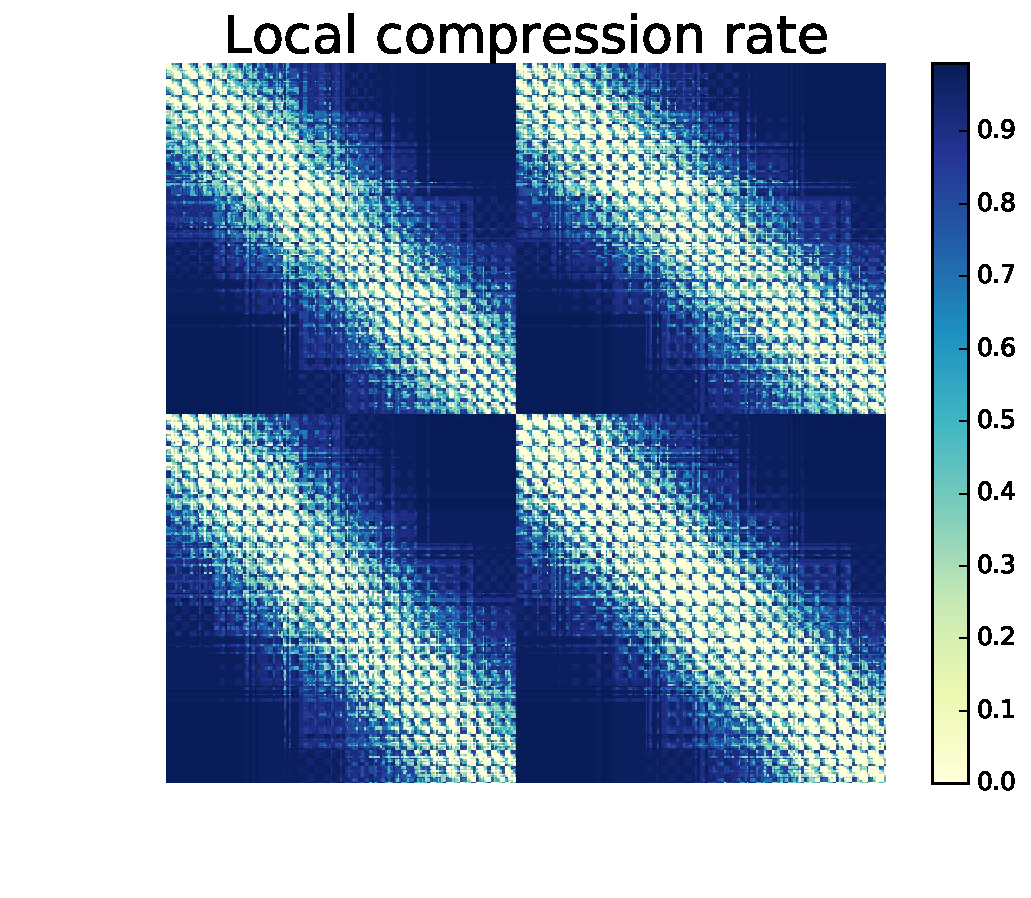
\includegraphics[width=.4\textwidth]{../images/graphe_mapp_output_local_comp_10_1_matrice450Fracs.pdf}} \\
\subfloat[][Errors and compression rates for different values of $\eta$ and $\varepsilon$.]
   {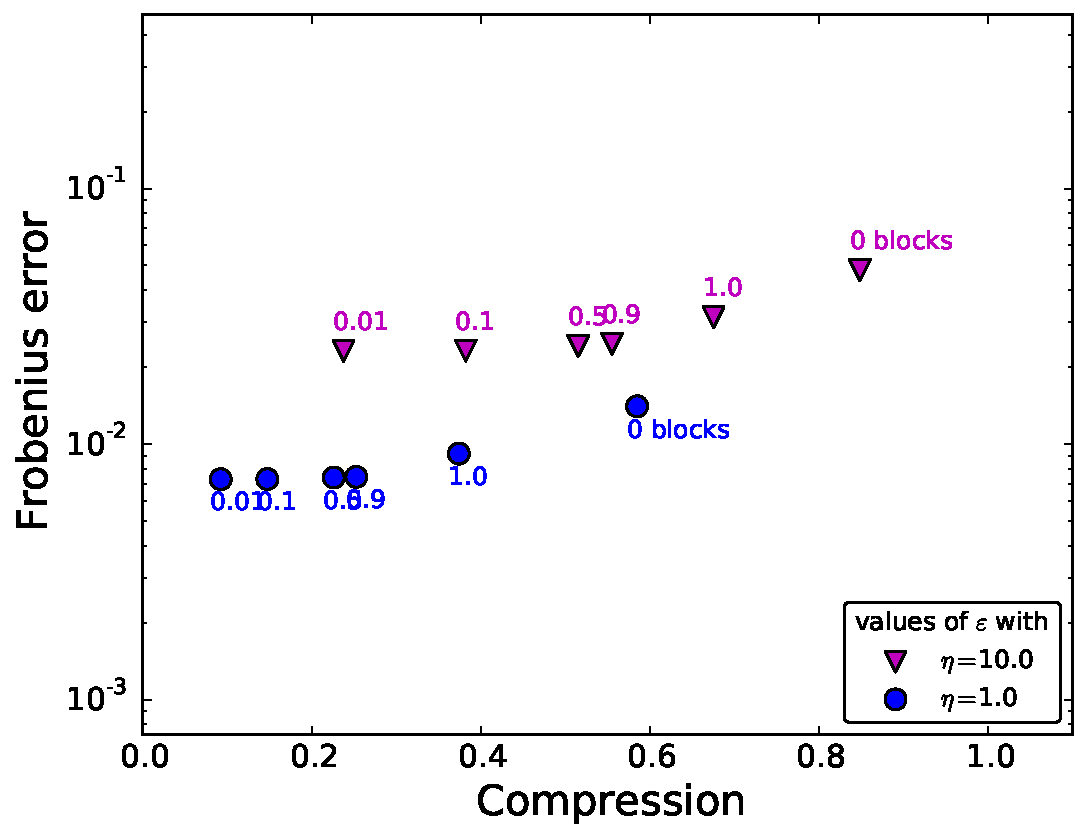
\includegraphics[width=.6\textwidth]{../images/graphe_compare_output_compression_18_08_2016matrice450Fracs.pdf}}
\caption{Results for the structure with $450$ fractures.}
\label{fig:450Fracs}
\end{figure}

\begin{figure}[p]
\centering
\subfloat[][Mesh.]
   {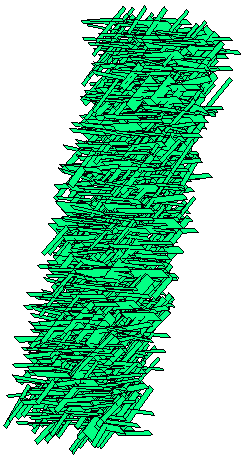
\includegraphics[width=.3\textwidth]{../images/visu_maillage1363Fracs.png}} \quad
\subfloat[][Matrix compression for $\eta=1, \varepsilon=0.9$.]
   {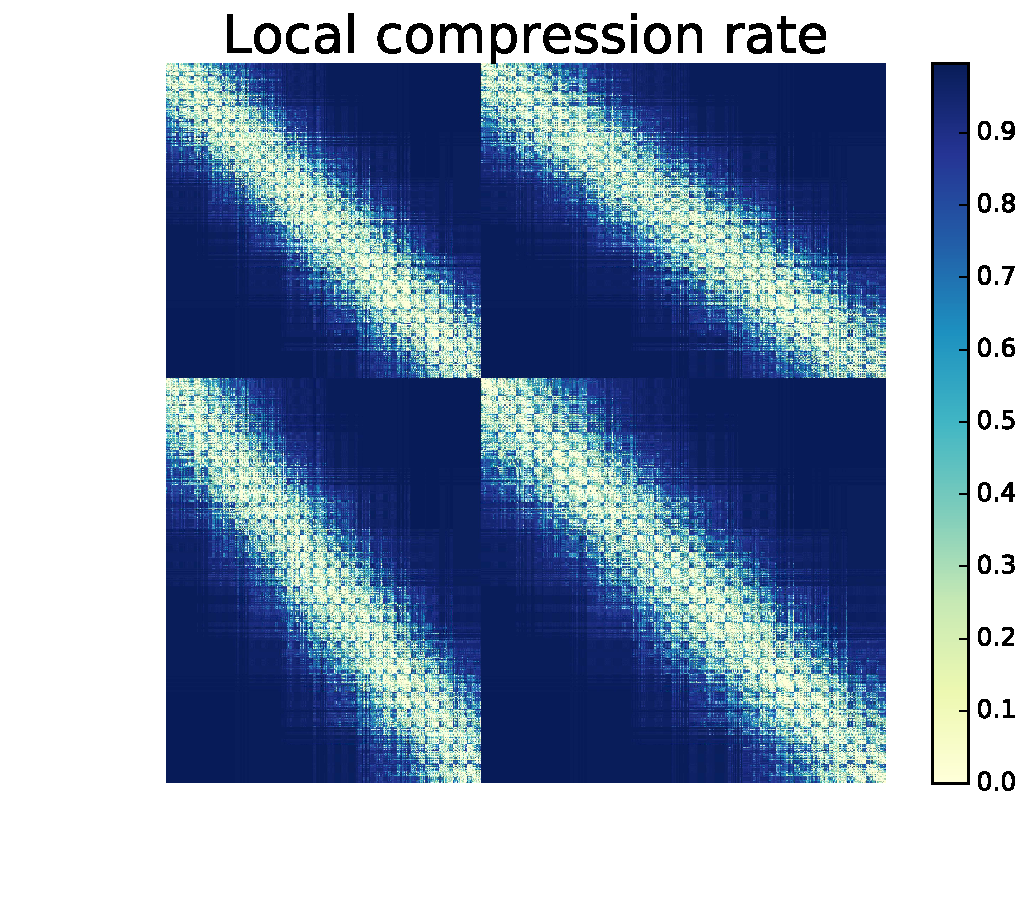
\includegraphics[width=.4\textwidth]{../images/graphe_mapp_output_local_comp_10_0,9_matrice1363Fracs.pdf}}\\
\subfloat[][Errors and compression rates for different values of $\eta$ and $\varepsilon$.]
   {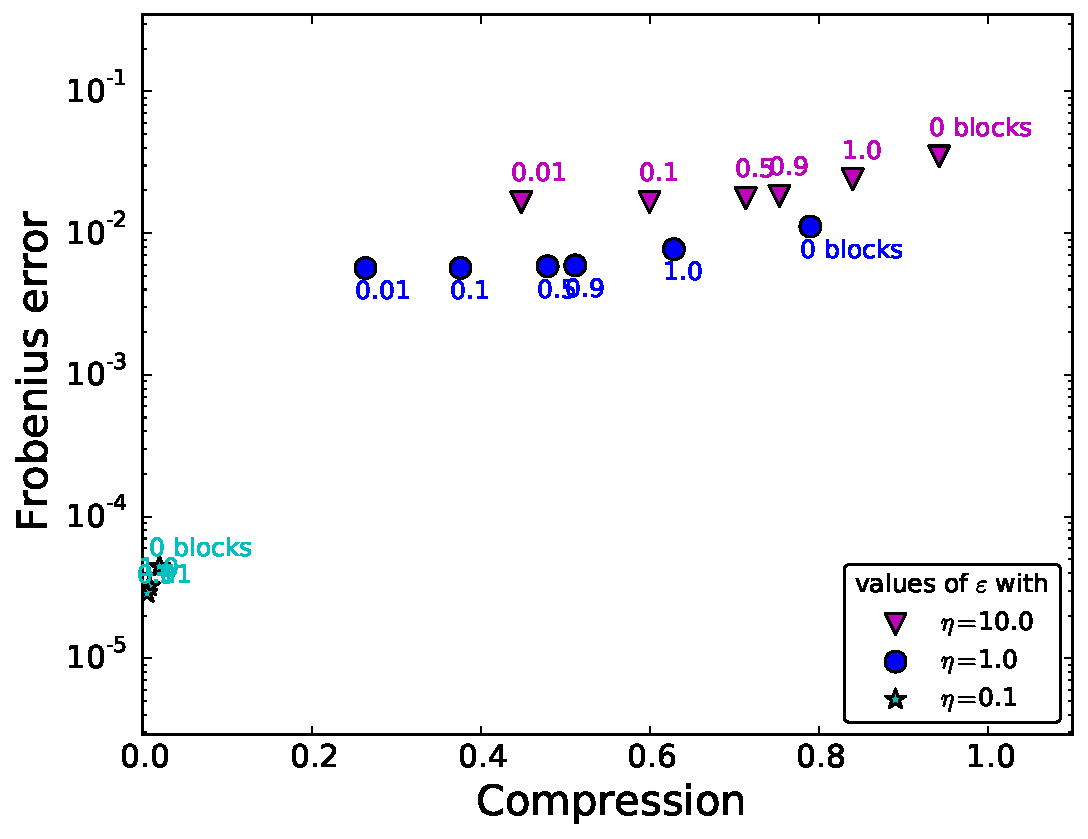
\includegraphics[width=.6\textwidth]{../images/graphe_compare_output_compression_18_08_2016matrice1363Fracs.pdf}}
\caption{Results for the structure with $1363$ fractures.}
\label{fig:1363Fracs}
\end{figure}

\begin{figure}[p]
\centering
\subfloat[][Mesh.]
   {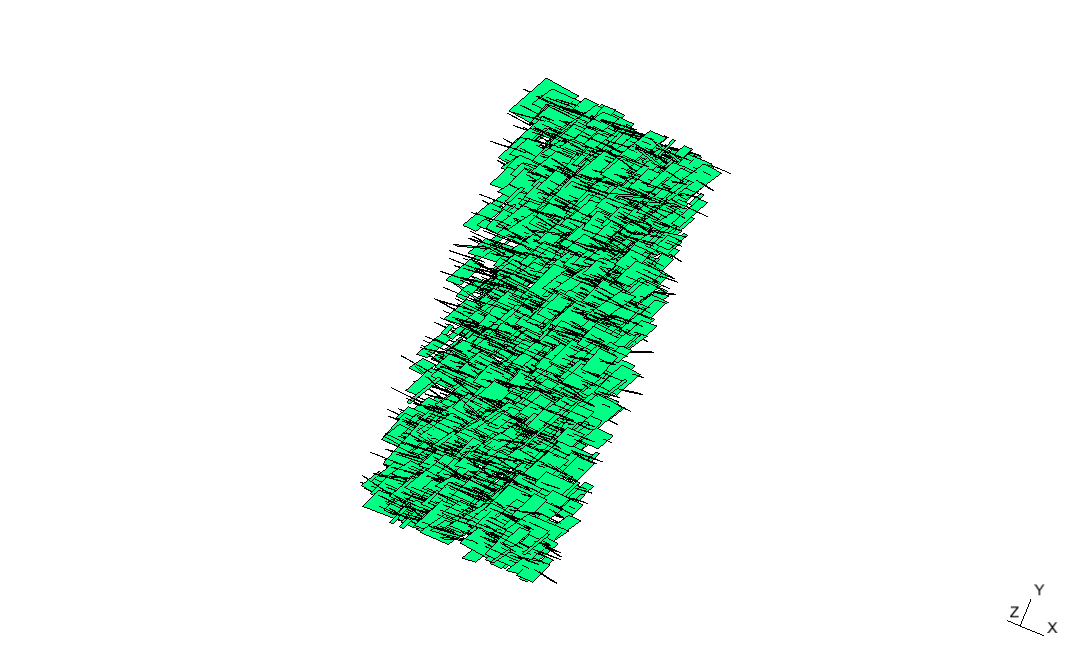
\includegraphics[width=.35\textwidth]{../images/visu_maillage1994Fracs.png}} 
\subfloat[][Errors and compression rates for different values of $\eta$ and $\varepsilon$.]
   {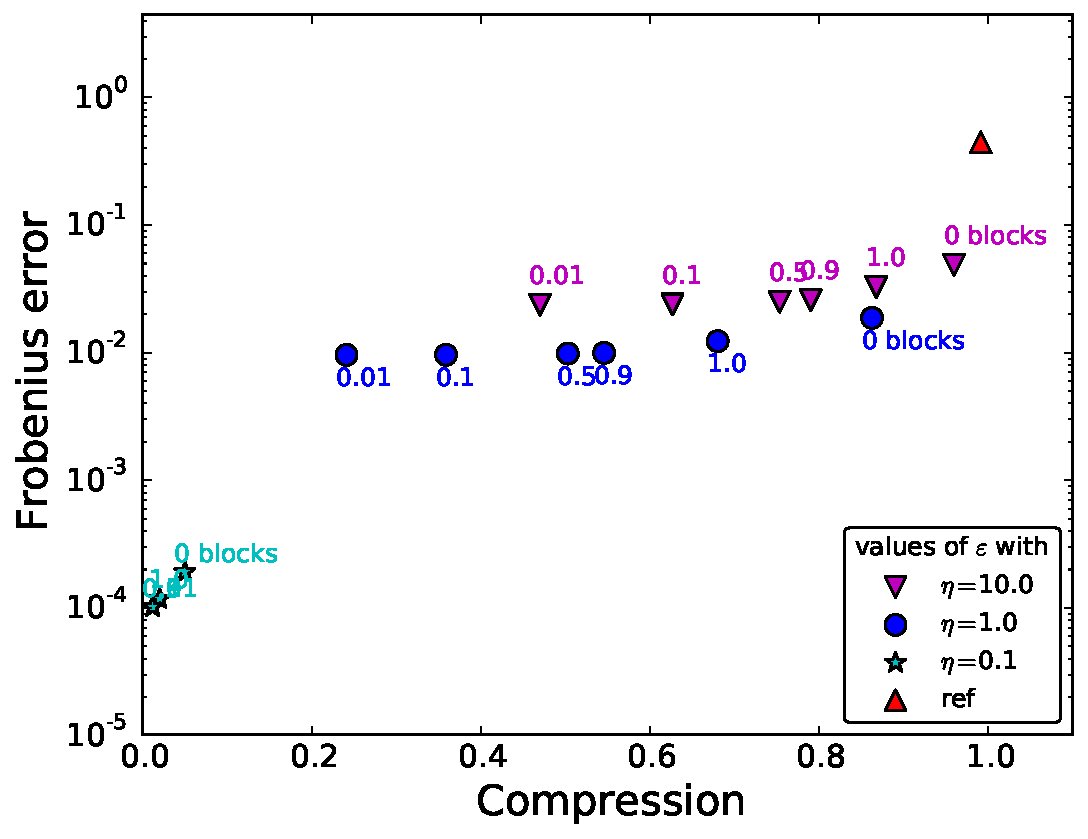
\includegraphics[width=.6\textwidth]{../images/graphe_compasparse_output_compression_18_08_2016matrice1994Fracs.pdf}}\\
\subfloat[][Times (s) to build the HM-ACA matrix and compression rates for different values of $\eta$ and $\varepsilon$.]
   {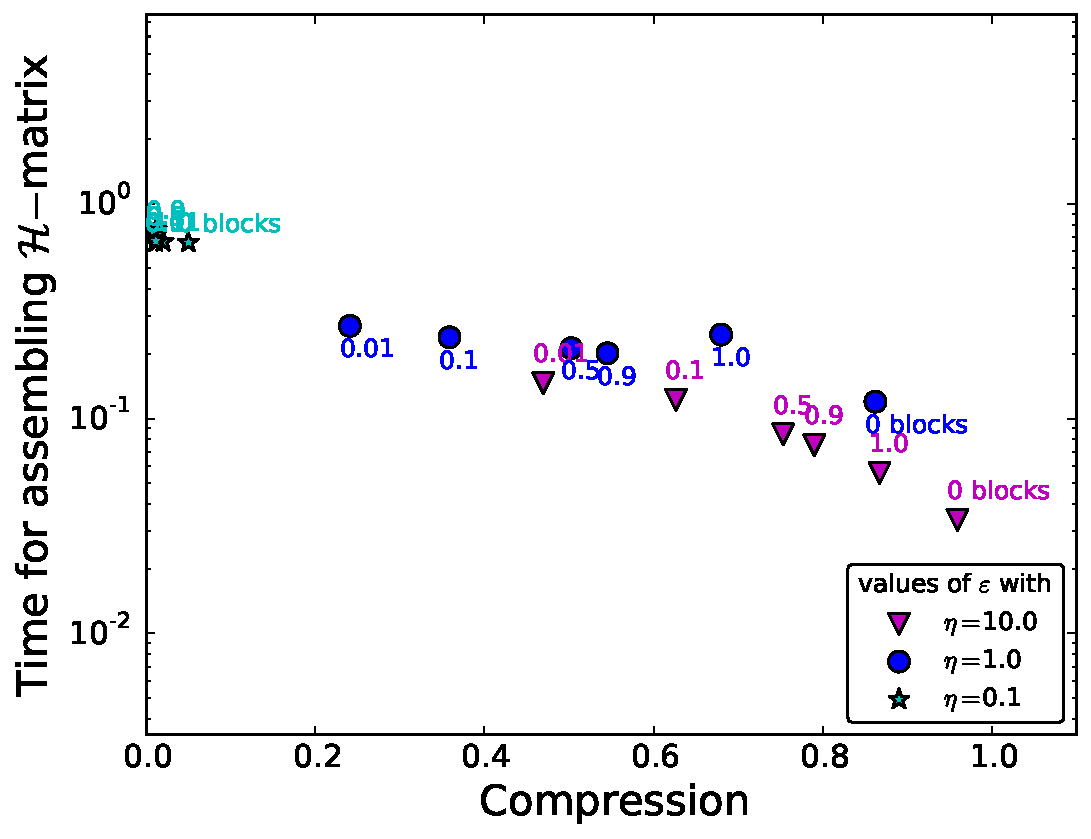
\includegraphics[width=.47\textwidth]{../images/graphe_tas_output_compression_18_08_2016matrice1994Fracs.pdf}} \;
\subfloat[][Times (s) to build the HM-ACA matrix and compression rates for different values of $\eta$ and $\varepsilon$.]
   {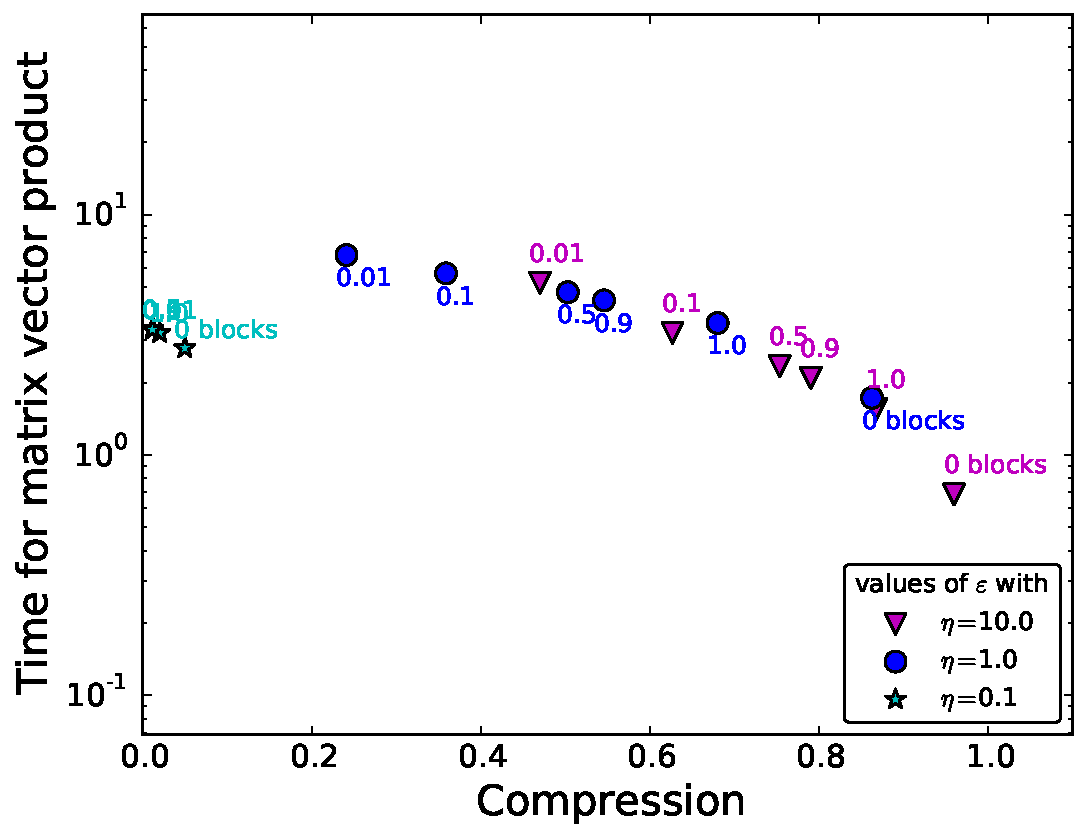
\includegraphics[width=.47\textwidth]{../images/graphe_tmv_output_compression_18_08_2016matrice1994Fracs.pdf}}
\caption{Results for the structure with $1994$ fractures.}
\label{fig:1994Fracs}
\end{figure}

\begin{figure}[p]
\centering
\subfloat[][Mesh.]
   {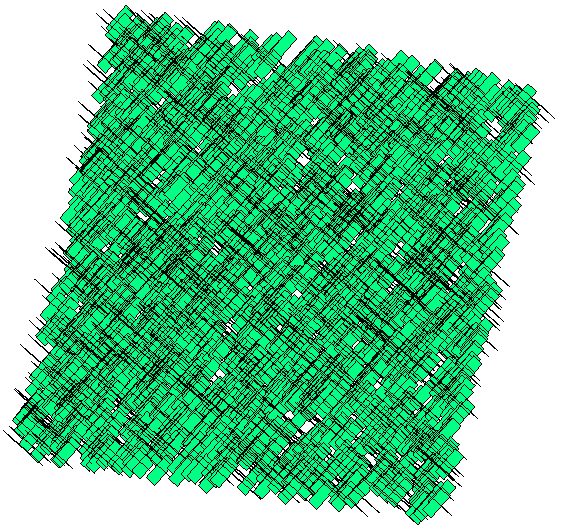
\includegraphics[width=.21\textwidth]{../images/visu_maillage2700FracsV1D1.png}} \qquad
\subfloat[][Errors and compression rates.] %for different values of $\eta$ and $\varepsilon$.]
   {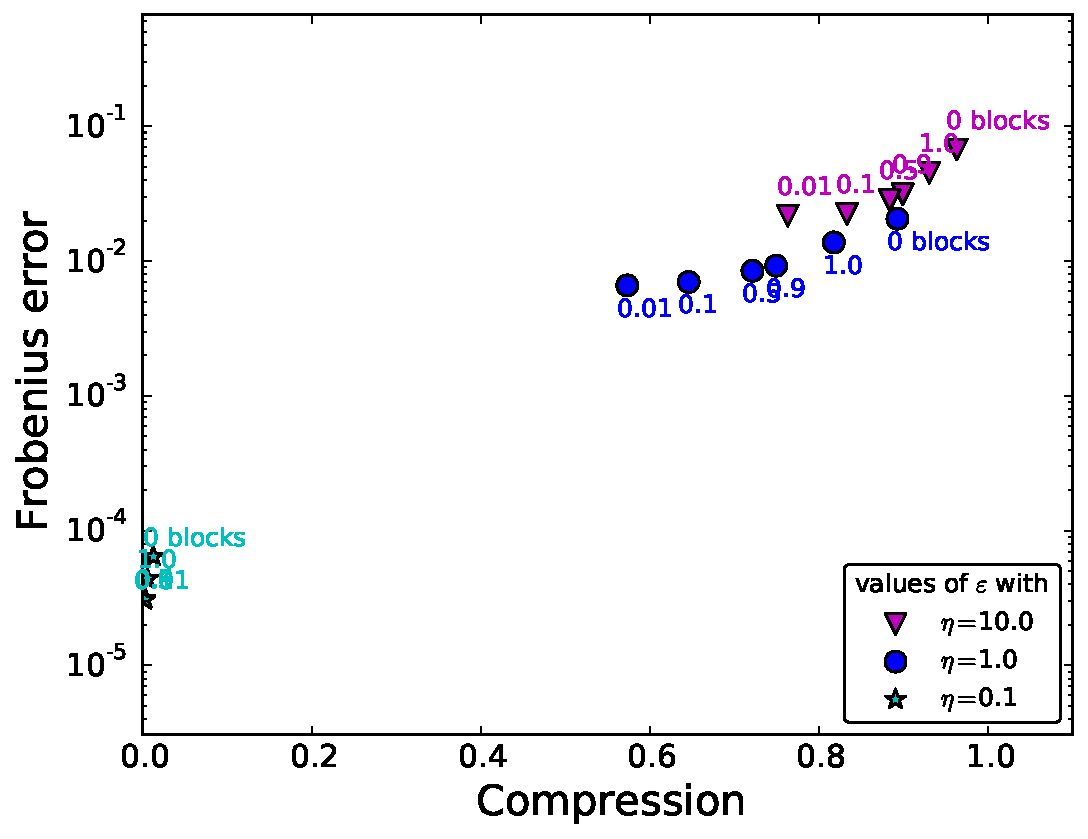
\includegraphics[width=.46\textwidth]{../images/graphe_compare_output_compression_18_08_2016matrice2700FracsV1D1.pdf}}
\caption{Results for the structure with $2700$ fractures inside a volume $V_1=300\times300\times20$.}
\label{fig:2700FracsV1D1}
\end{figure}

\begin{figure}[p]
\centering
\subfloat[][Mesh.]
   {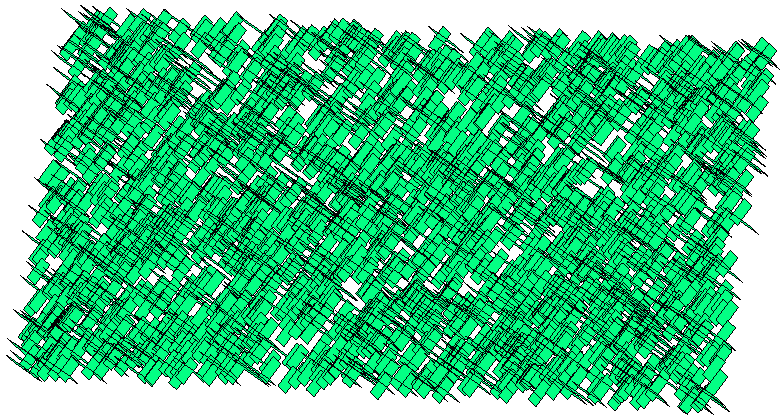
\includegraphics[width=.36\textwidth]{../images/visu_maillage2700FracsV2D2.png}} \qquad
\subfloat[][Errors and compression rates.] %for different values of $\eta$ and $\varepsilon$.]
   {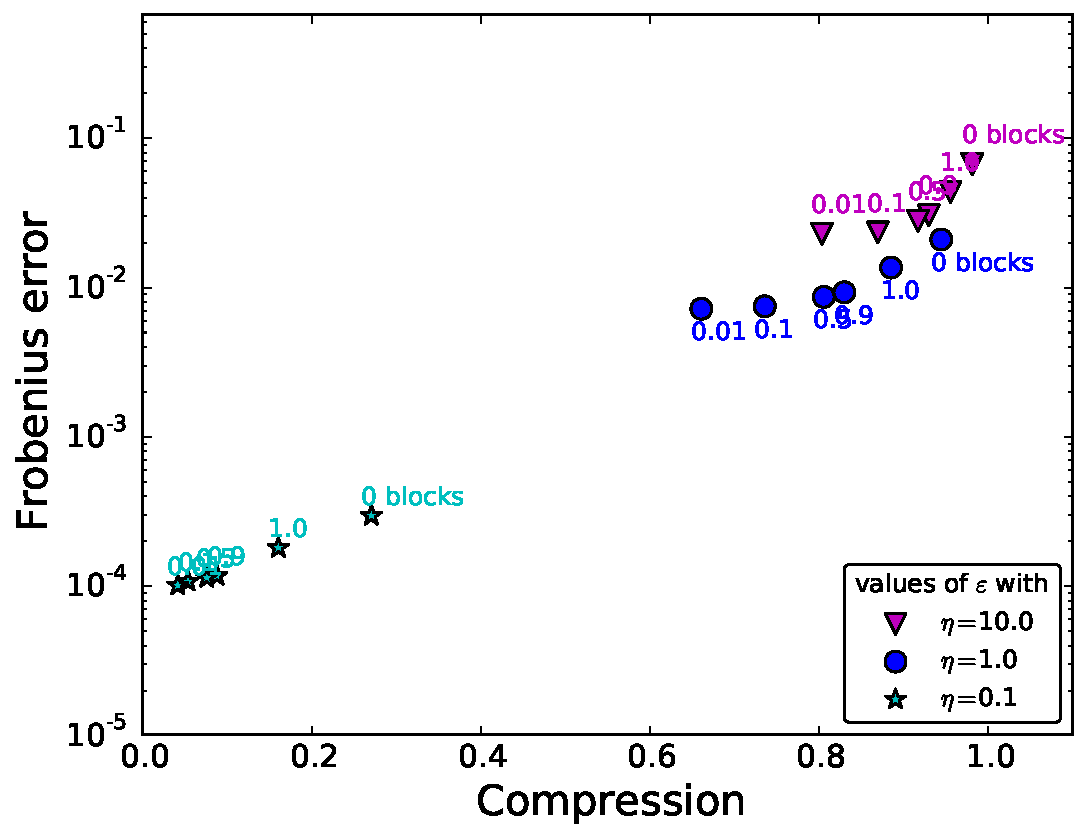
\includegraphics[width=.46\textwidth]{../images/graphe_compare_output_compression_18_08_2016matrice2700FracsV2D2.pdf}}
\caption{Results for the structure with $2700$ fractures inside a volume $V_2=600\times300\times20$.}
\label{fig:2700FracsV2D2}
\end{figure}

\begin{figure}[p]
\centering
\subfloat[][Mesh.]
   {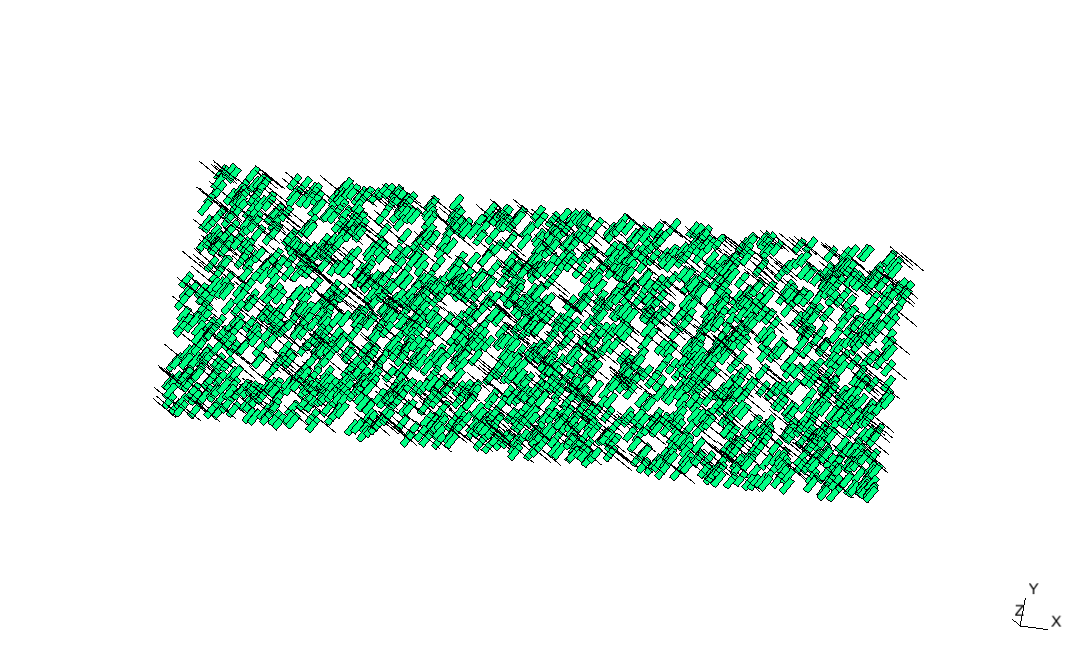
\includegraphics[width=.539\textwidth]{../images/visu_maillage2700FracsV3D3.png}}
\subfloat[][Errors and compression rates.] %for different values of $\eta$ and $\varepsilon$.]
   {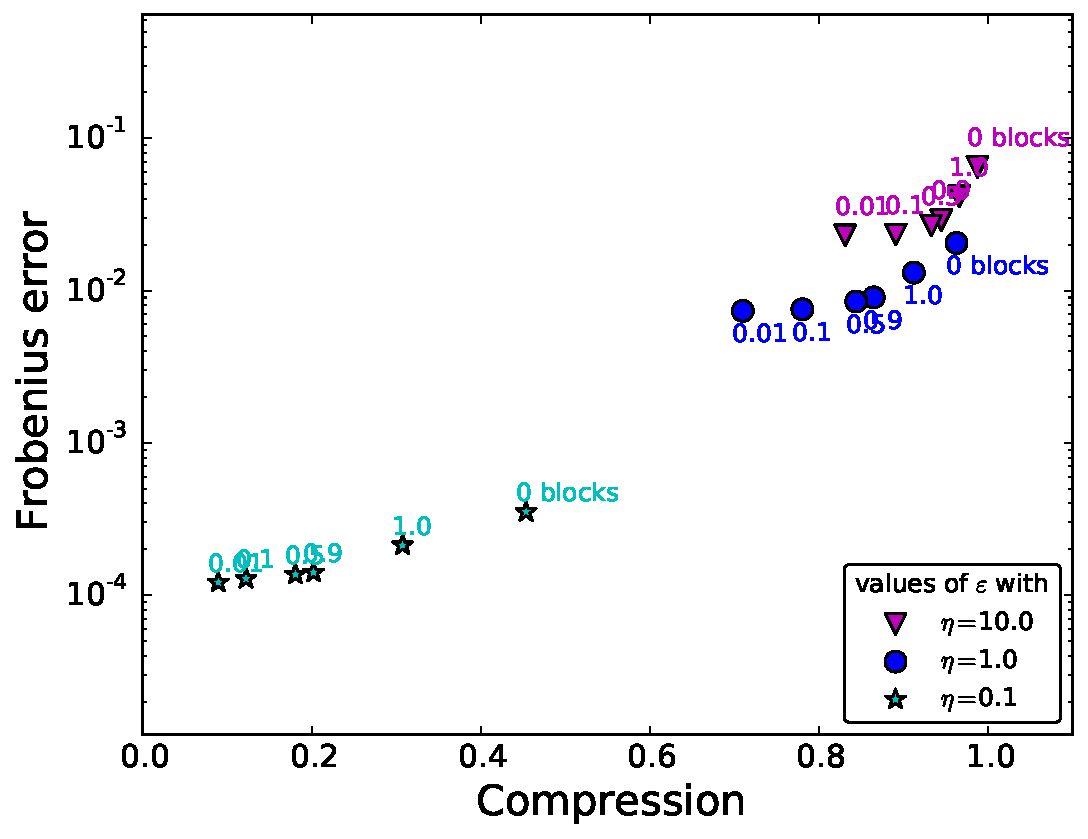
\includegraphics[width=.46\textwidth]{../images/graphe_compare_output_compression_18_08_2016matrice2700FracsV3D3.pdf}}
\caption{Results for the structure with $2700$ fractures inside a volume $V_3=900\times300\times20$.}
\label{fig:2700FracsV3D3}
\end{figure}


\begin{figure}[p]
\centering
\subfloat[][Mesh.]
   {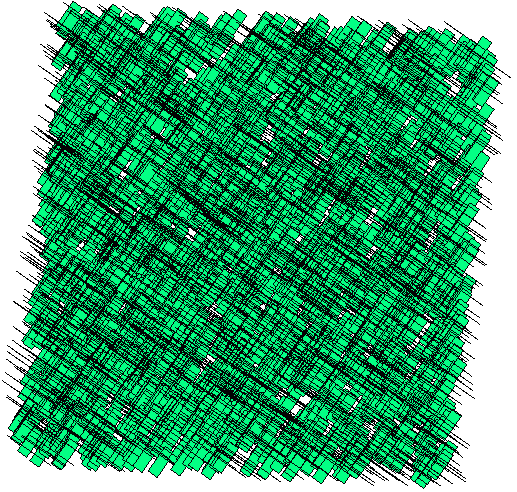
\includegraphics[width=.21\textwidth]{../images/visu_maillage3600FracsV1DN1.png}} \qquad
\subfloat[][Errors and compression rates.] %for different values of $\eta$ and $\varepsilon$.]
   {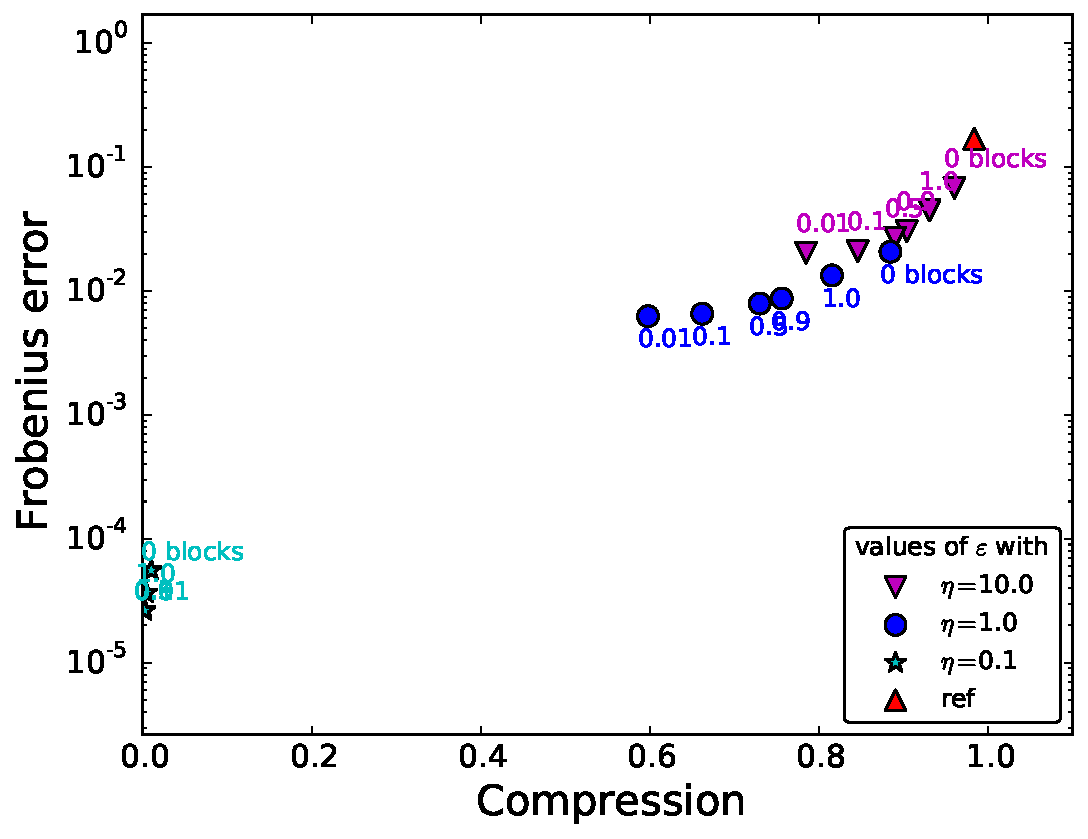
\includegraphics[width=.46\textwidth]{../images/graphe_compasparse_output_compression_18_08_2016matrice3600FracsV1DN1.pdf}}
\caption{Results for the structure with $3600$ fractures inside a volume $V_1=300\times300\times20$.}
\label{fig:3600FracsV1DN1}
\end{figure}

\begin{figure}[p]
\centering
\subfloat[][Mesh.]
   {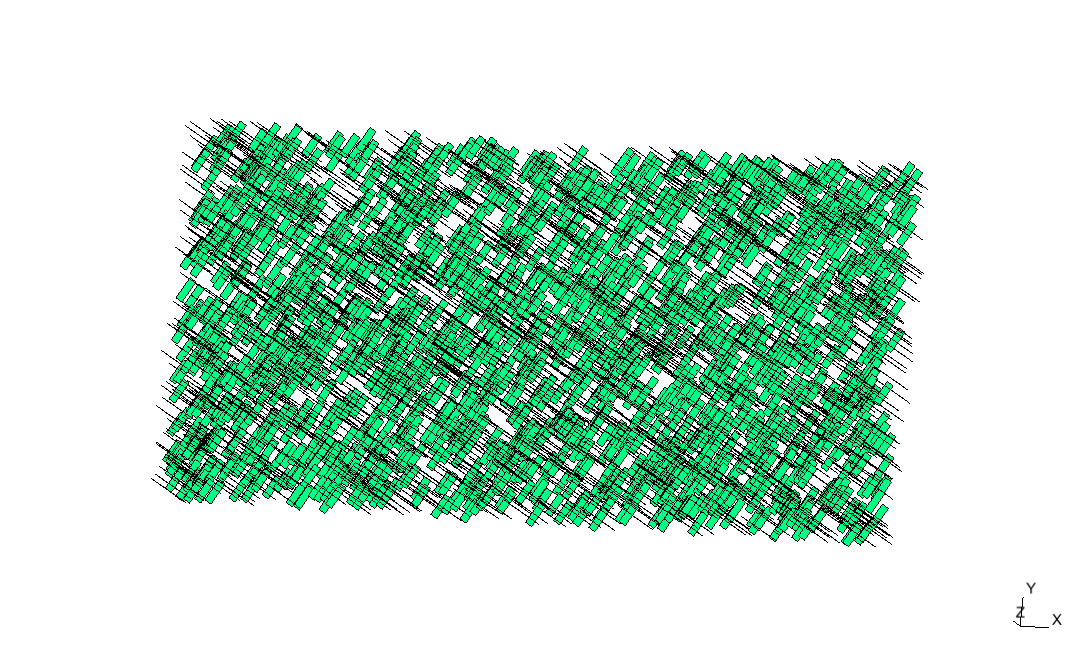
\includegraphics[width=.36\textwidth]{../images/visu_maillage3600FracsV2DN2.png}} \qquad
\subfloat[][Errors and compression rates.] %for different values of $\eta$ and $\varepsilon$.]
   {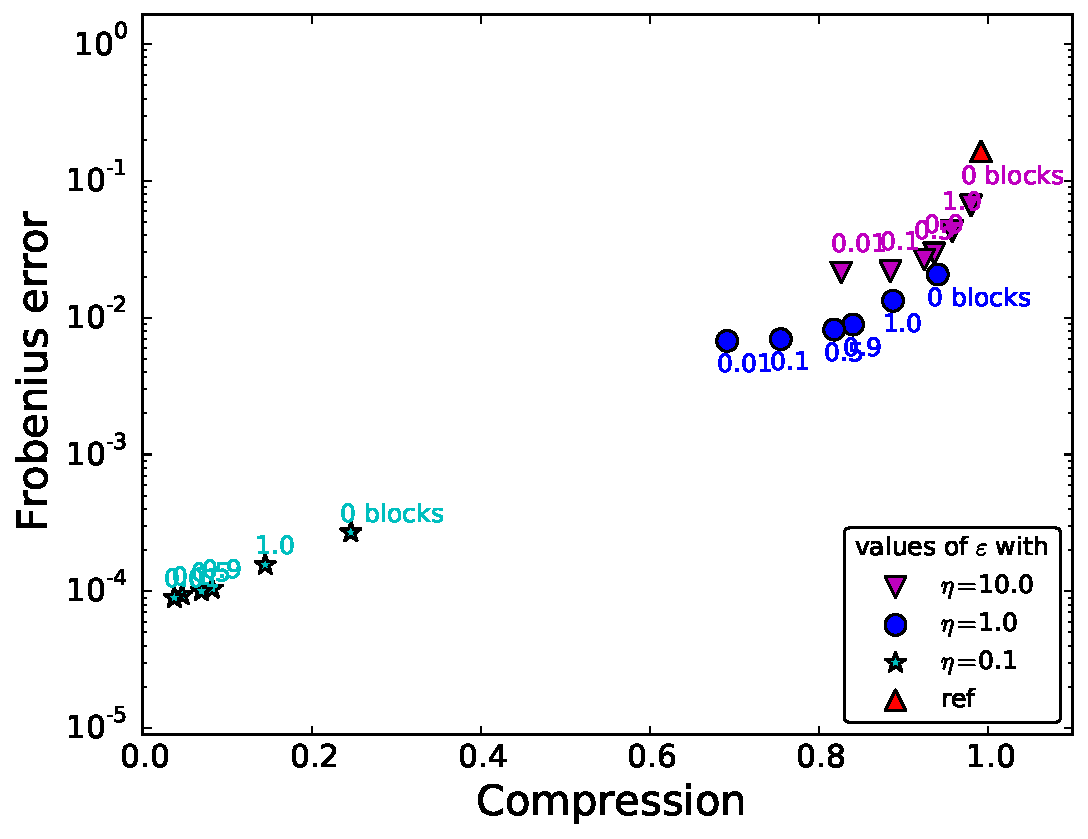
\includegraphics[width=.46\textwidth]{../images/graphe_compasparse_output_compression_18_08_2016matrice3600FracsV2DN2.pdf}}
\caption{Results for the structure with $3600$ fractures inside a volume $V_2=600\times300\times20$.}
\label{fig:3600FracsV2DN2}
\end{figure}

\begin{figure}[p]
\centering
\subfloat[][Mesh.]
   {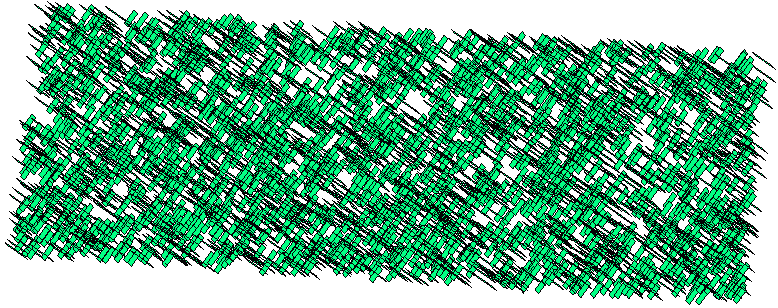
\includegraphics[width=.539\textwidth]{../images/visu_maillage3600FracsV3DN3.png}}
\subfloat[][Errors and compression rates.] %for different values of $\eta$ and $\varepsilon$.]
   {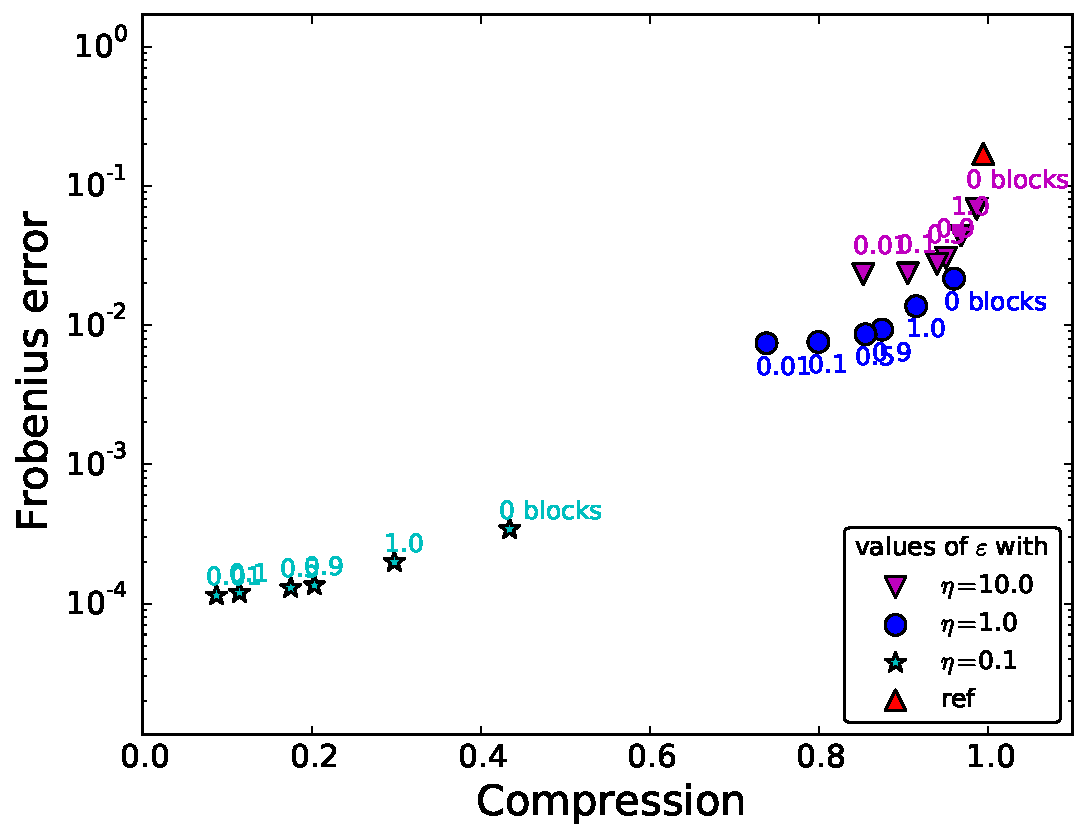
\includegraphics[width=.46\textwidth]{../images/graphe_compasparse_output_compression_18_08_2016matrice3600FracsV3DN3.pdf}}
\caption{Results for the structure with $3600$ fractures inside a volume $V_3=900\times300\times20$.}
\label{fig:3600FracsV3DN3}
\end{figure}


\begin{figure}[p]
\centering
\subfloat[][Mesh.]
   {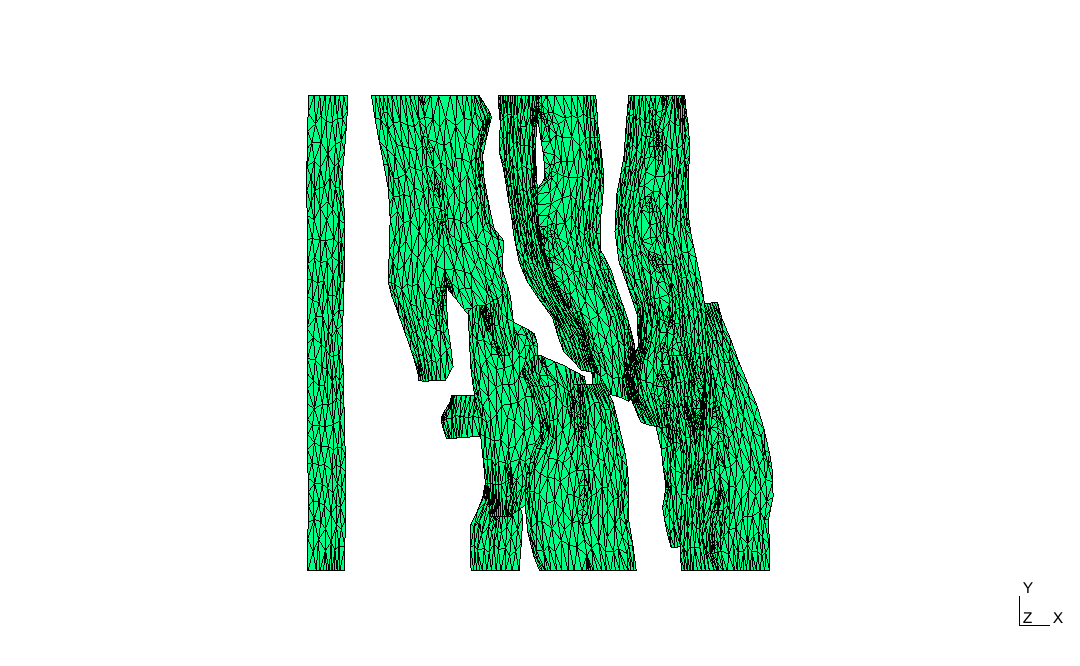
\includegraphics[width=.41\textwidth]{../images/visu_maillage5364FracsTriangles.png}}
\subfloat[][Errors and compression rates for different values of $\eta$ and $\varepsilon$.]
   {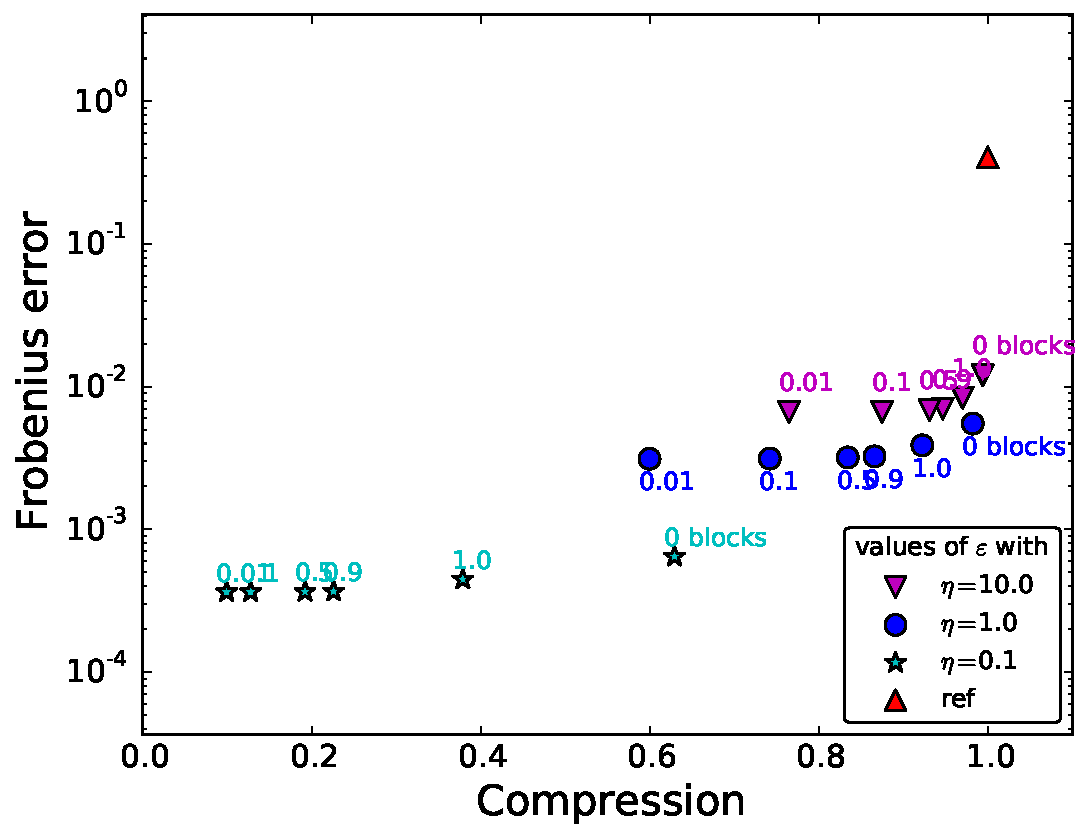
\includegraphics[width=.58\textwidth]{../images/graphe_compasparse_output_compression_18_08_2016matrice5364FracsTriangles.pdf}}\\
\subfloat[][Times (s) to build the HM-ACA matrix and compression rates for different values of $\eta$ and $\varepsilon$.]
   {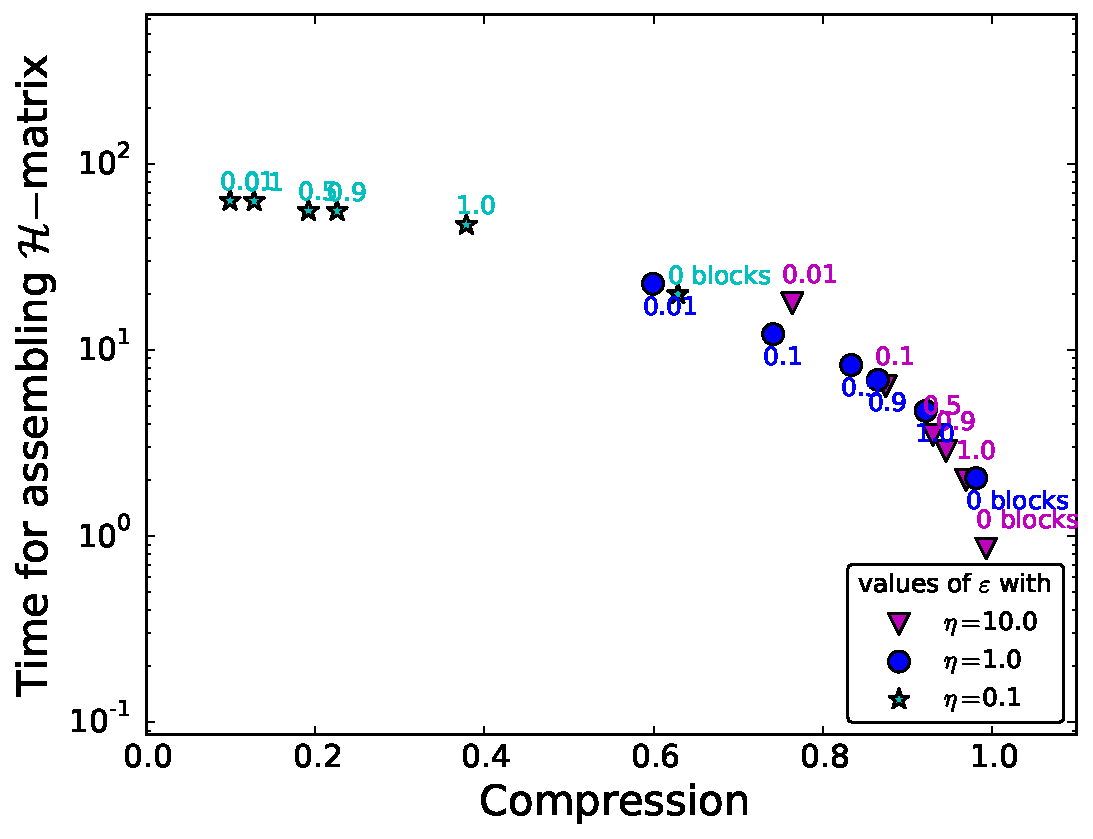
\includegraphics[width=.47\textwidth]{../images/graphe_tas_output_compression_18_08_2016matrice5364FracsTriangles.pdf}} \;
\subfloat[][Times (s) to build the HM-ACA matrix and compression rates for different values of $\eta$ and $\varepsilon$.]
   {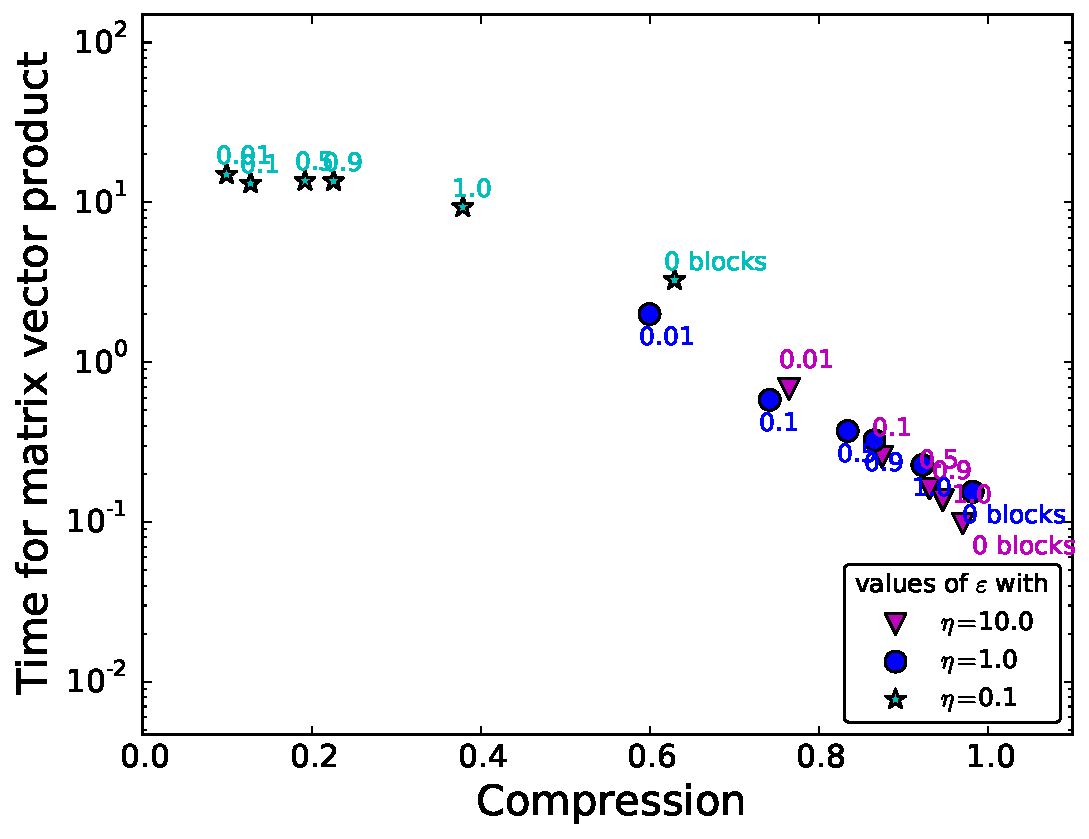
\includegraphics[width=.47\textwidth]{../images/graphe_tmv_output_compression_18_08_2016matrice5364FracsTriangles.pdf}}
\caption{Results for the structure of faults with $5364$ fractures.}
\label{fig:5364FracsTriangles}
\end{figure}



